\documentclass[12pt]{beamer}
%\documentclass[20pt,handout]{beamer}
\usetheme{Darmstadt}
\usepackage{graphicx}
%\usepackage[german]{babel}
\usepackage[T1]{fontenc}
\usepackage[utf8]{inputenc}
\usepackage{tikz}
\setbeamertemplate{footline}[frame number]

\newcommand{\cc}[1]{\includegraphics[height=4mm]{img/#1.png}}
\usepackage{ifthen}
\newcommand{\license}[2][]{\\#2\ifthenelse{\equal{#1}{}}{}{\\\scriptsize\url{#1}}}
\usepackage{textcomp}

\pgfdeclareimage[height=.6cm]{c3d2logo}{./img/c3d2.pdf} 


\pgfdeclarelayer{foreground}
\pgfsetlayers{main,foreground}
\logo{\pgfputat{\pgfxy(-1,0)}{\pgfbox[center,base]{\pgfuseimage{c3d2logo}}}}


\title{NSA, Prism und co - Wie schützt man sich vor Überwachung?}
\author{\small Marius Melzer \& Stephan Thamm\\\large Chaos Computer Club Dresden}
\date{22.01.2014}

\begin{document}
\maketitle

\section{Einleitung}
\subsection{}

\begin{frame}
  \frametitle{Wer sind wir?}
  \begin{figure}
    
\includegraphics[height=0.7\textheight]{img/fingerabdruck.jpg}
  \end{figure}
\end{frame}

\begin{frame}
  \frametitle{Wer sind wir?}
  \begin{figure}
    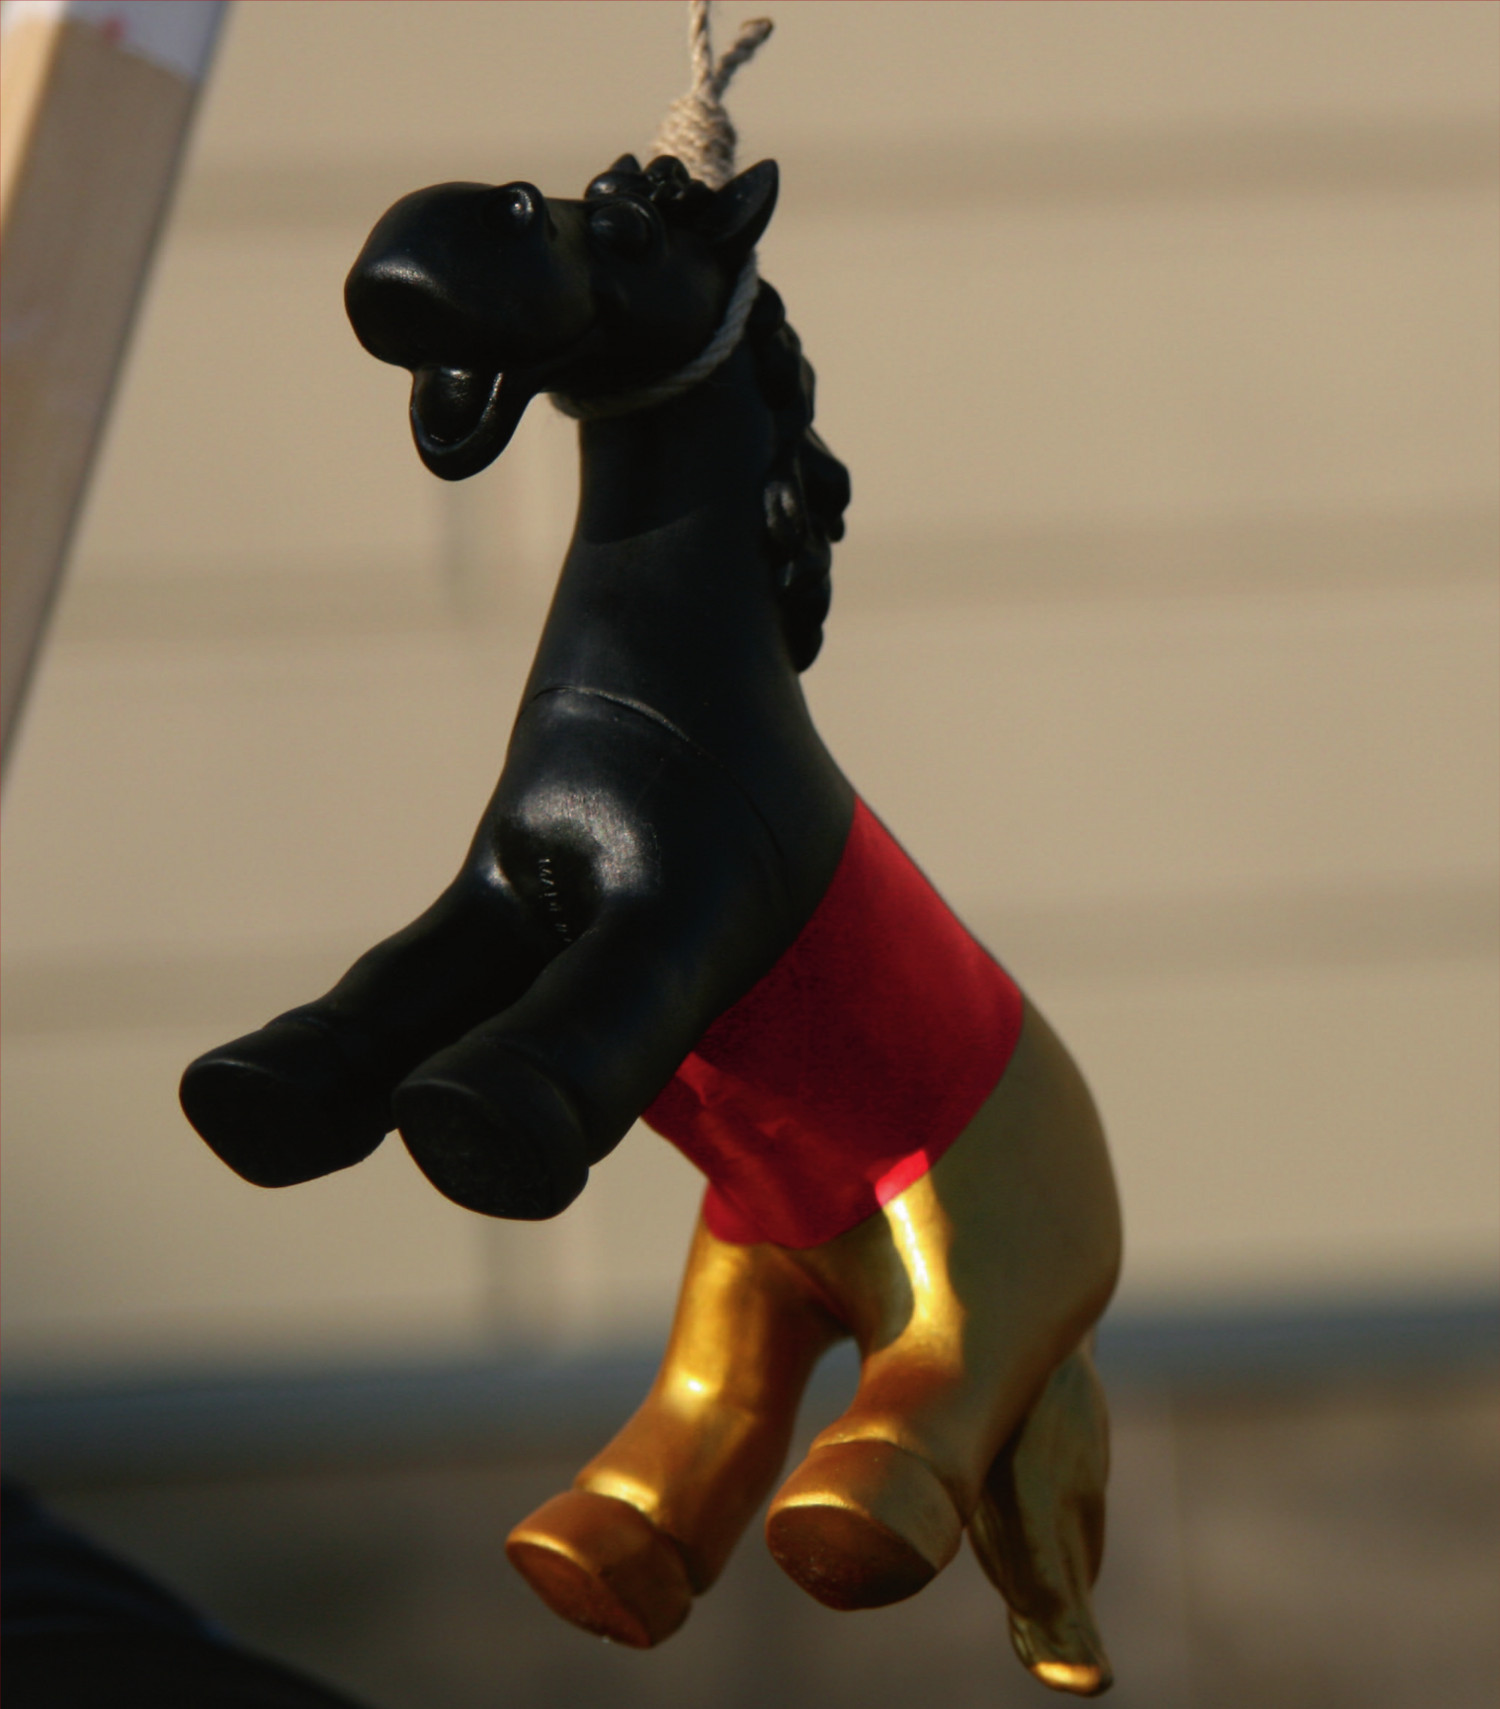
\includegraphics[height=0.7\textheight]{img/trojaner.jpg}
  \end{figure}
\end{frame}

\begin{frame}
    \frametitle{Wer sind wir?}
    \begin{itemize}
      \item<1-> Chaos Computer Club Dresden (\url{http://c3d2.de})
          \note{}
      \item<2-> Datenspuren: Herbst 2014 \url{http://datenspuren.de}
      \item<3-> Podcasts (\url{http://pentamedia.de})
      \item<4-> Chaos macht Schule
    \end{itemize}
\end{frame}

\begin{frame}
    \frametitle{Bundespräsident Gauck zur NSA-Überwachung}
    \begin{center}
      "`Wir wissen z.B., dass es nicht so ist, wie bei der Stasi und dem KGB, dass es dicke Aktenbände gibt, wo unsere Gesprächsinhalte alle aufgeschrieben und schön abgeheftet sind. Das ist es nicht."'
      \end{center}
\end{frame}

\begin{frame}
    \frametitle{Stasi vs. NSA}
    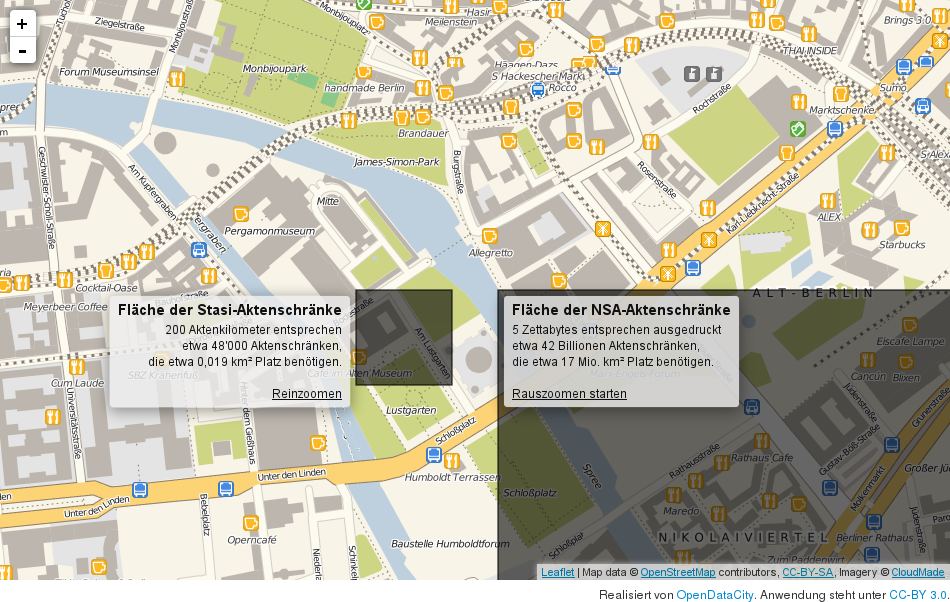
\includegraphics[height=0.7\textheight]{img/akten1.png}
\end{frame}

\begin{frame}
    \frametitle{Stasi vs. NSA}
    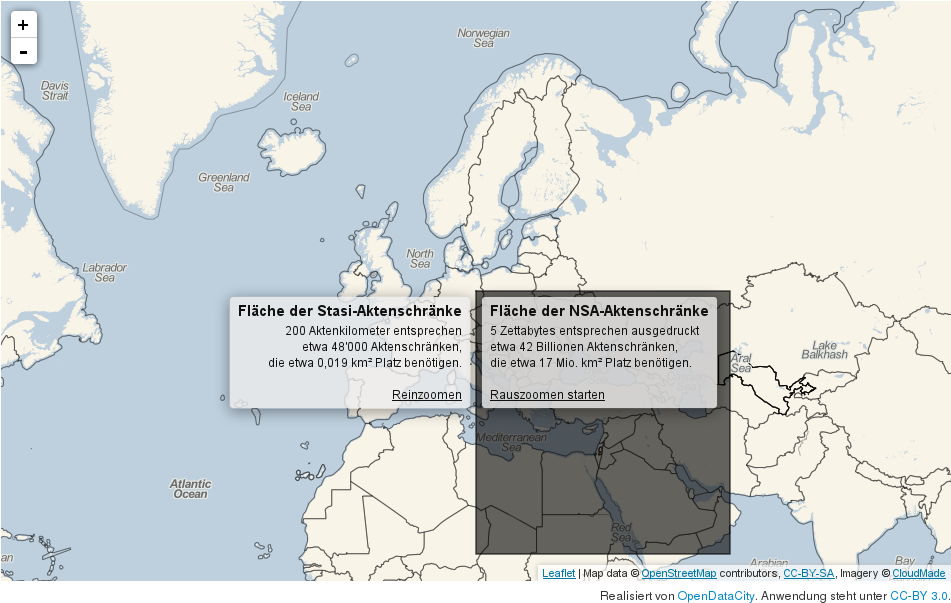
\includegraphics[height=0.7\textheight]{img/akten2.png}
\end{frame}

\begin{frame}
    \frametitle{Merkels Handy}
    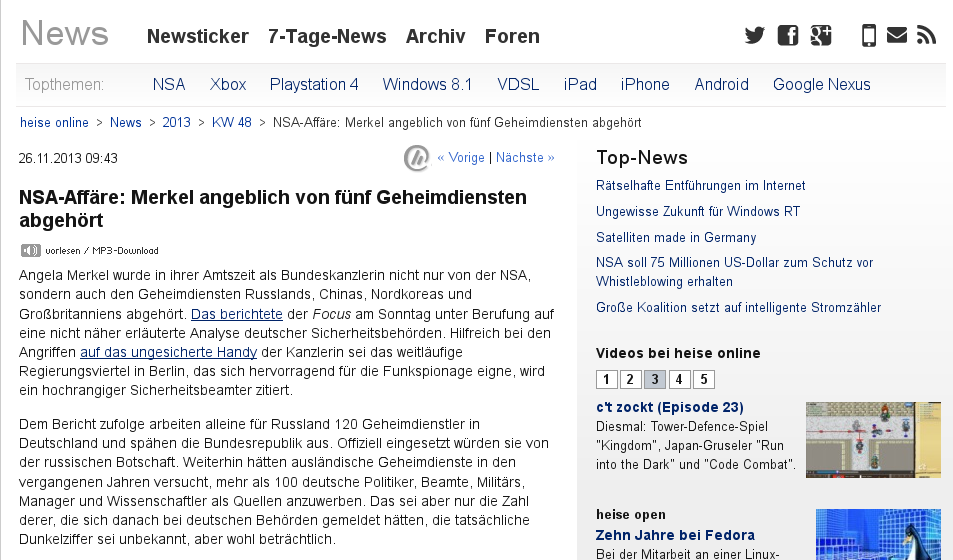
\includegraphics[height=0.7\textheight]{img/heise-merkel.png}
\end{frame}

\section{Tempora}
\subsection{}

\begin{frame}
    \frametitle{Tempora}
    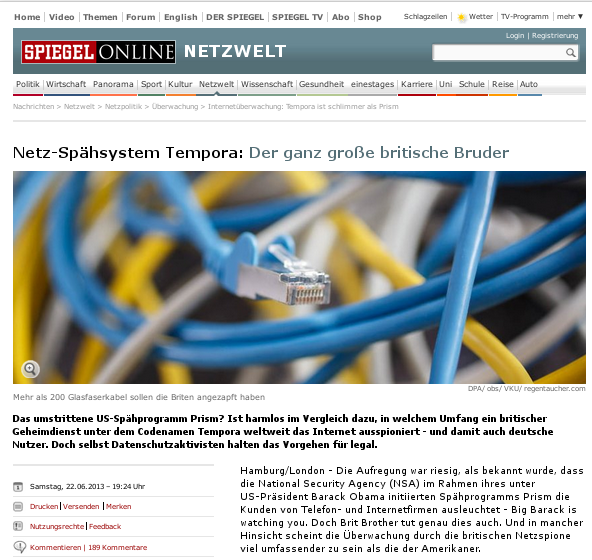
\includegraphics[height=0.7\textheight]{img/spiegel-tempora.png}
\end{frame}

\begin{frame}
    \frametitle{Verschlüsselung}
    \includegraphics[height=0.7\textheight]<2->{img/asym_encryption.png}
\end{frame}

\begin{frame}
    \frametitle{SSL / TLS}
    \begin{itemize}
      \item<2-> SSL = Secure Socket Layer
      \item<3-> eingesetzt im Web, Mail, ...
      \item<4-> hierarchische Struktur
      \item<5-> gespeicherte Liste von vertrauenswürdigen Zertifikaten
    \end{itemize}
\end{frame}

\begin{frame}
    \frametitle{Von Firefox vertraute Zertifikate}
    \begin{center}
      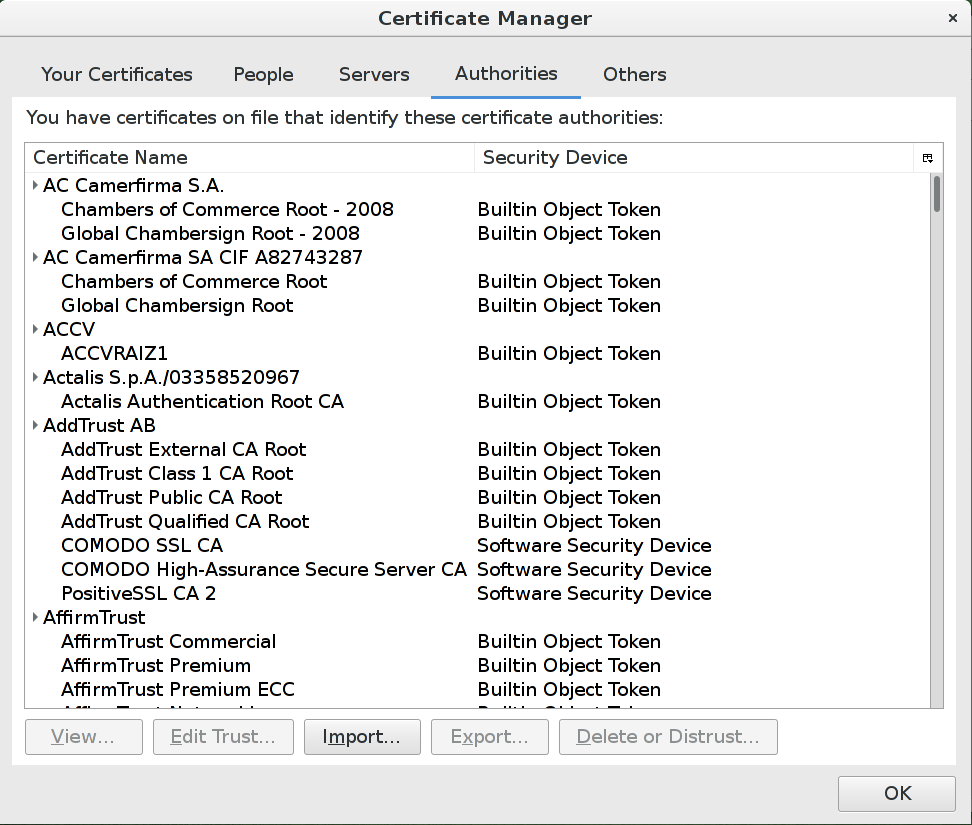
\includegraphics[height=5cm]{img/zertifikate.png}
    \end{center}
\end{frame}

\begin{frame}
  \frametitle{HTTPS Everywhere}
    \begin{center}
      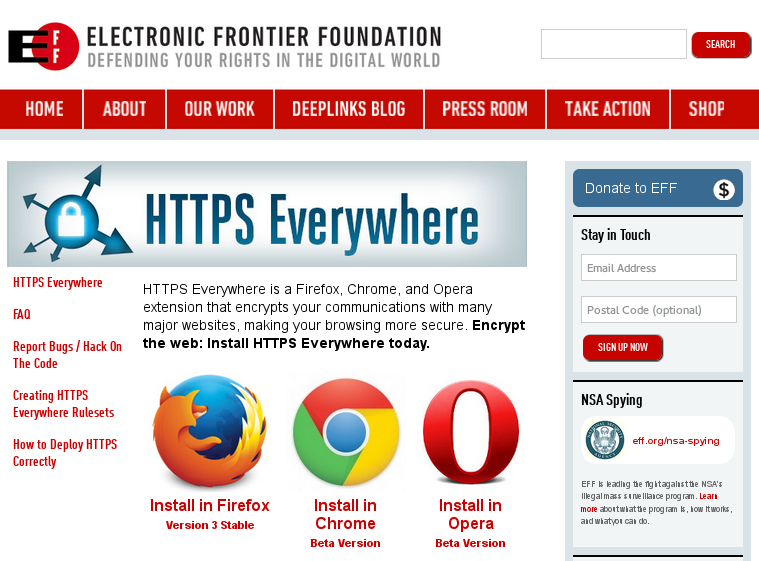
\includegraphics[height=5cm]{img/https-everywhere.png}
    \end{center}
\end{frame}

\section{Prism}
\subsection{}

\begin{frame}
    \frametitle{Prism}
    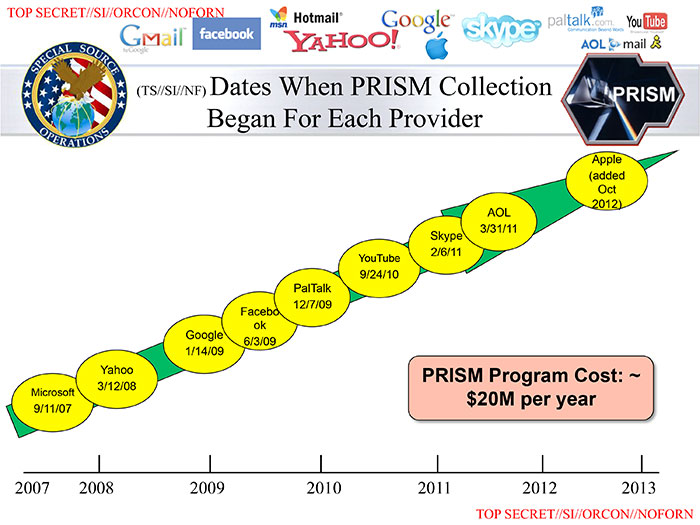
\includegraphics[height=0.7\textheight]{img/prism.jpg}
\end{frame}

\begin{frame}
  \frametitle{Dezentrale Dienste}
    \begin{itemize}
      \item<2-> Email
      \item<3-> Jabber
      \item<4-> Bitmessage
      \item<5-> palava.tv
    \end{itemize}
\end{frame}

\begin{frame}
    \frametitle{Lavabit}
    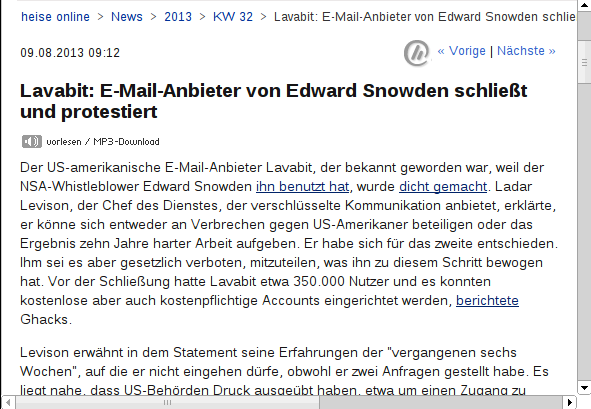
\includegraphics[height=0.6\textheight]{img/heise_lavabit.png}
\end{frame}

\begin{frame}
    \frametitle{Ende-zu-Ende-Verschlüsselung I}
    \begin{itemize}\Large
      \item Email: GPG = Gnu Privacy Guard
      \item Thunderbird: Enigmail
      \item Outlook: Gpg4win
      \item Web: Mailvelope (Firefox, Chrome)
      \item Alternative: Bitmessage
    \end{itemize}
\end{frame}

\begin{frame}
  \frametitle{Ende-zu-Ende-Verschlüsselung II}
  \begin{itemize}
    \item<2-> OTR für Jabber:
      \begin{itemize}
        \item Pidgin mit OTR-Plugin für Linux und Windows
        \item GibberBot oder Xabber für Android
        \item Adium für Mac, ChatSecure für iOS
      \end{itemize}
    \item<3-> palava.tv für Videotelefonie
    \item<4-> Redphone für Handytelefonate (Android)
    \item<5-> TextSecure für SMS (Android)
  \end{itemize}
\end{frame}

\section{Vorratsdatenspeicherung}
\subsection{}

\begin{frame}
  \frametitle{Vorratsdatenspeicherung (USA)}
    \begin{center}
      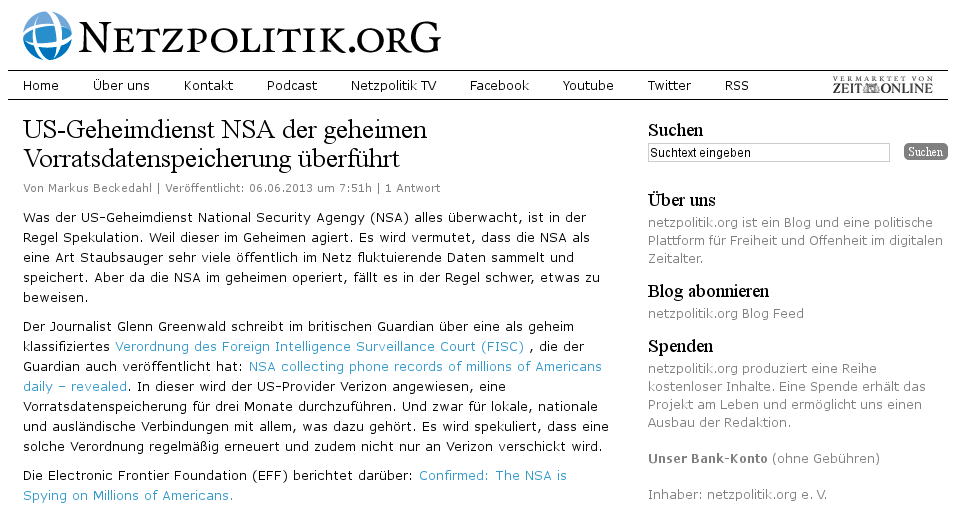
\includegraphics[height=5cm]{img/netzpolitik-verizon.png}
    \end{center}
\end{frame}

\begin{frame}
  \frametitle{Vorratsdatenspeicherung (Deutschland)}
    \begin{center}
      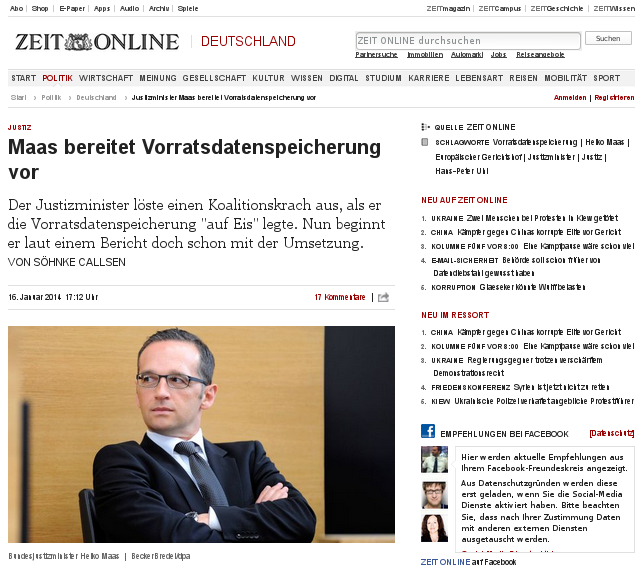
\includegraphics[height=5cm]{img/zeit-vds.png}
    \end{center}
\end{frame}

\begin{frame}
  \frametitle{Metadaten}
  \begin{itemize}
    \item<2-> Handynetz
      \begin{itemize}
        \item<3-> Telefonnummern
        \item<4-> Zeitpunkt und Dauer (Telefonate, SMS)
        \item<5-> Funkzelle (Ort)
      \end{itemize}
    \item<6->Internet
      \begin{itemize}
        \item<7-> IP-Adresse
        \item<8-> Alle Verbindungen
        \item<9-> Email: Adressen von Sender und Empfänger, Zugriff
      \end{itemize}
  \end{itemize}
\end{frame}

\begin{frame}
  \frametitle{Metadaten}
    \begin{center}
      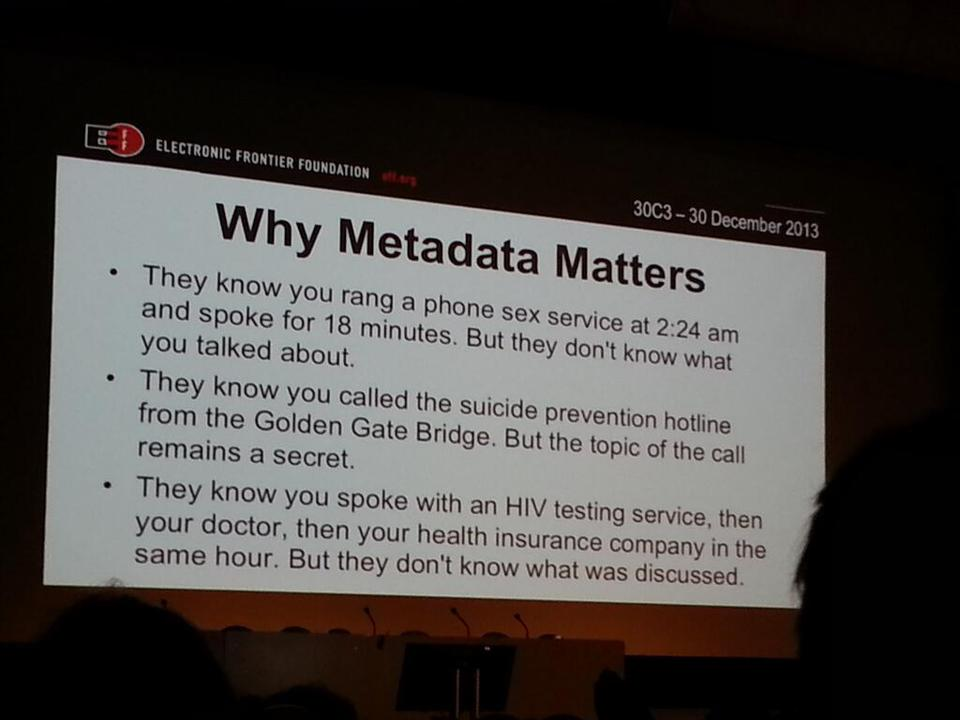
\includegraphics[height=5cm]{img/metadata-matters.jpg}
    \end{center}
\end{frame}

\begin{frame}
    \frametitle{Metadaten}
    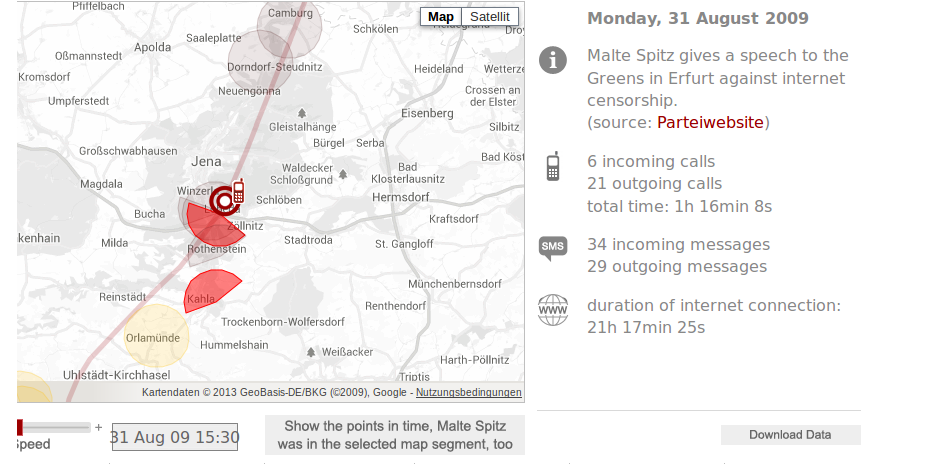
\includegraphics[height=0.7\textheight]{img/maltespitz.png}
\end{frame}

\begin{frame}
    \frametitle{Lightbeam}
    \begin{center} \Large Lightbeam \end{center}
\end{frame}

\begin{frame}
    \frametitle{Disconnect.me}
    \begin{center} \Large Disconnect.me \end{center}
\end{frame}

\begin{frame}
    \frametitle{Tor}
    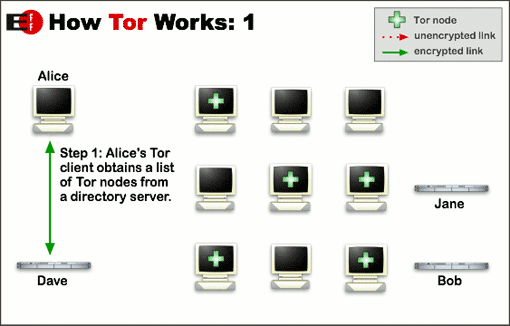
\includegraphics[height=0.7\textheight]{img/tor1.png}
    \\{\small \href{https://www.torproject.org/images/htw1.png}{Grafik}: \href{https://creativecommons.org/licenses/by/3.0/us/}{\cc{by}} The Tor Project}
\end{frame}

\begin{frame}
    \frametitle{Tor}
    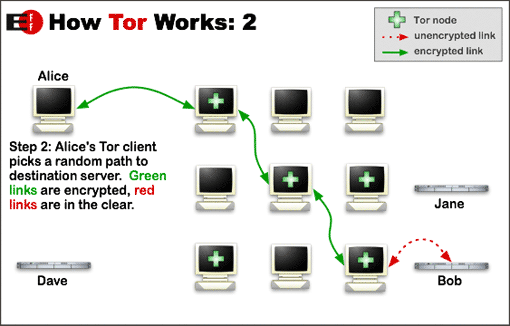
\includegraphics[height=0.7\textheight]{img/tor2.png}
    \\{\small \href{https://www.torproject.org/images/htw2.png}{Grafik}: \href{https://creativecommons.org/licenses/by/3.0/us/}{\cc{by}} The Tor Project}
\end{frame}

\begin{frame}
    \frametitle{Tor}
    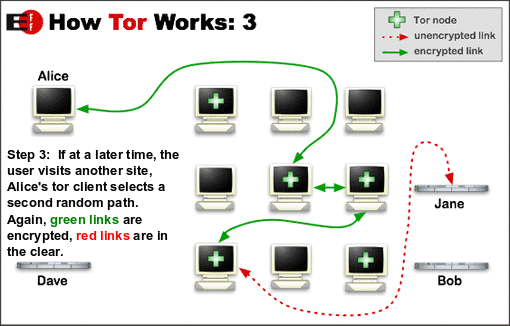
\includegraphics[height=0.7\textheight]{img/tor3.png}
    \\{\small \href{https://www.torproject.org/images/htw3.png}{Grafik}: \href{https://creativecommons.org/licenses/by/3.0/us/}{\cc{by}} The Tor Project}
\end{frame}

\section{Verhalten}
\subsection{}

\begin{frame}
    \frametitle{Datensparsamkeit}
    \begin{itemize}
        \item<2-> Viele Daten zusammen ergeben Profile
        \item<3-> Werden die Daten gebraucht?
        \item<4-> Werden echte Daten gebraucht?
            \begin{itemize}
              \item<5-> Pseudonymität
              \item<6-> mailinator.com
            \end{itemize}
    \end{itemize}
\end{frame}

\begin{frame}
    \frametitle{Passwörter}
    \begin{itemize}
        \item<2-> Keine einfachen Wörter
        \item<3-> Groß-, Kleinbuchstaben, Ziffern, Sonderzeichen
        \item<4-> Beispiele:
            \begin{itemize}
                \item<5-> dragon
                \item<6-> (nCuAj.§Tsm!f
                \item<7-> IchLiebeDich
                \item<8-> .§)=")=`
                \item<9-> 123456
                \item<10-> qwerty
                \item<11-> Mks?o/.u,1Psw!
            \end{itemize}
        \item<12-> Verschiedene Passwörter nutzen!
    \end{itemize}
\end{frame}

\begin{frame}
    \frametitle{Wie schütze ich meinen Computer?}
    \begin{itemize}
      \item Virenscanner
      \item Firewall
      \item Aktuelle und vertrauenswürdige Software
    \end{itemize}
\end{frame}

\begin{frame}
    \frametitle{Wie schütze ich mein Smartphone?}
    \begin{itemize}
      \item Permissions
      \item Firewall (z.B. AFwall+)
      \item Aktuelle und vertrauenswürdige Software
    \end{itemize}
\end{frame}

\begin{frame}
    \frametitle{Freie Software}
    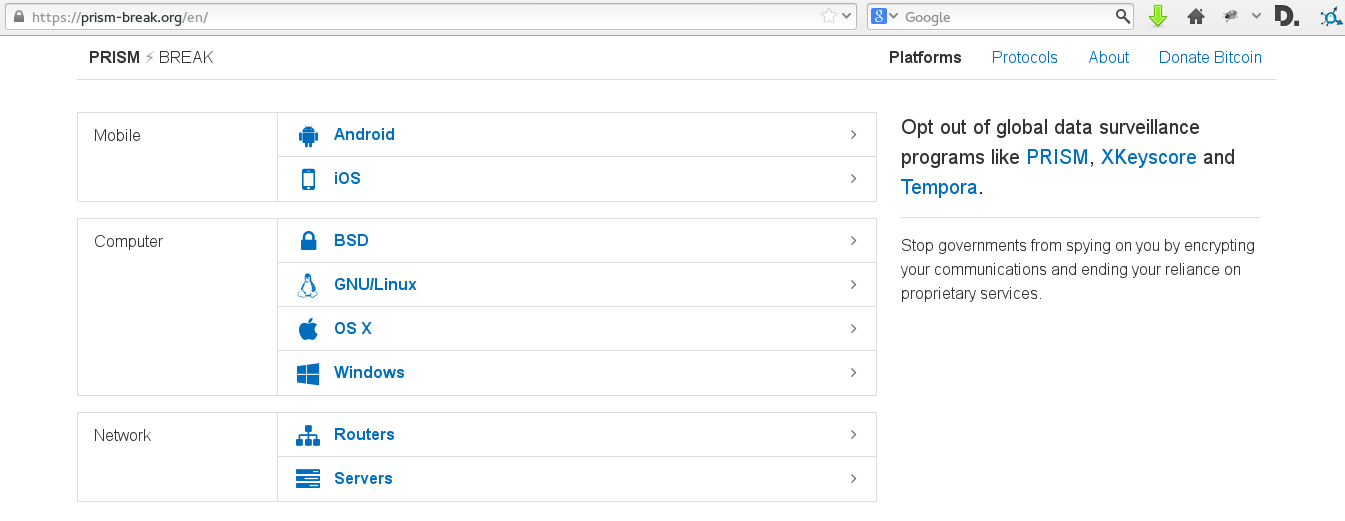
\includegraphics[height=0.7\textheight]{img/prism-break1.png}
\end{frame}

\begin{frame}
    \frametitle{Freie Software}
    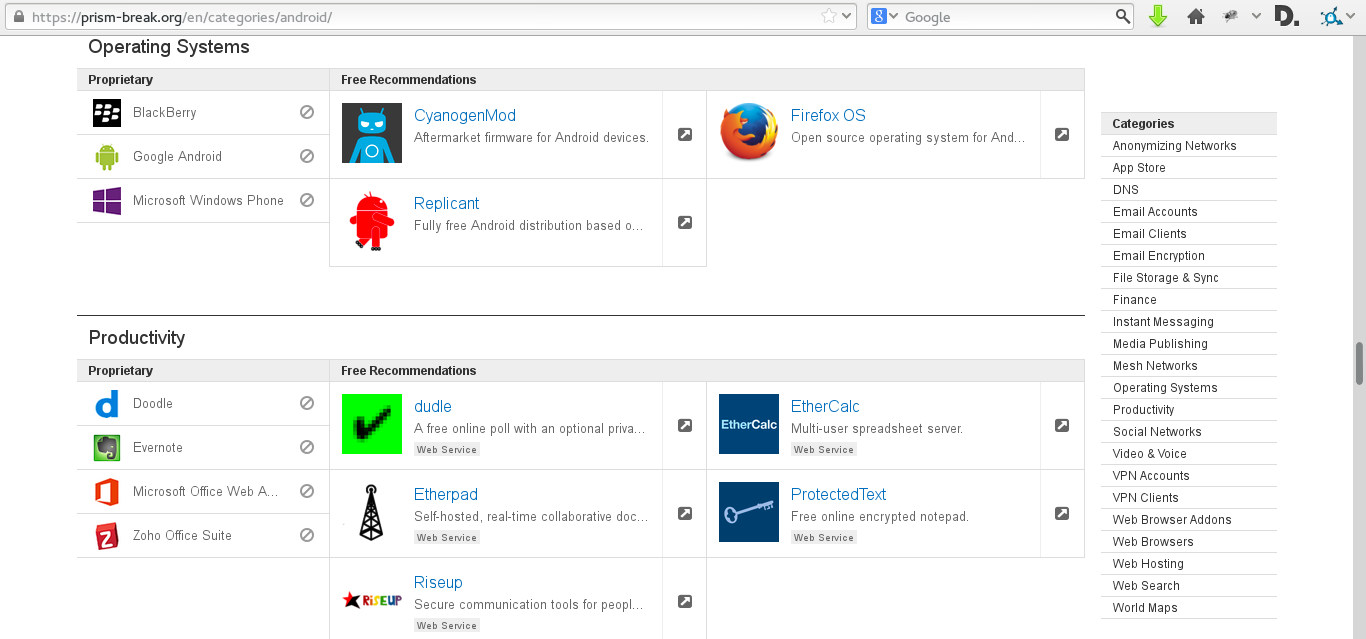
\includegraphics[height=0.7\textheight]{img/prism-break2.png}
\end{frame}

\begin{frame}
    \frametitle{Diskussion}
    \begin{center} {\Large Diskussion}\\Marius Melzer und Stephan Thamm\\CMS Dresden: schule@c3d2.de \end{center}
\end{frame}

\end{document}
